\clearpage\secrel{o\F}\secdown

And now we have all classes required to build basic \F\ system.

\bigskip\noindent
\emph{We will not follow any standards of language}. Our goal is to do a long
jump from an assembly-like language for a dumb stack-based virtual machine
\ref{FVM}\ to metasystem optimized for modern challenges: distributed cluster
and cloud computers, production data systems, huge multiformat websites,
dynamic compilers for a lot of target platforms including embedded, IoT and
mobile devices (\emph{Android in the first place}). There are a huge amount of
experimental features, whilst \F\ standards emanate stinks of antique,
naphthalene and oblivion. But the core idea of language stays the same.

\secrel{\F\ Virtual Machine}\label{FVM}\secdown

Classical \F\ has:
\begin{itemize}[nosep]
  \item \emph{CPU} commands without attributes, manipulates data on
  \item \emph{data stack}, which resides in
  \item \emph{main memory} with lot of call/ret commands use separate
  \item \emph{return stack}
\end{itemize}

\noindent
As we move to pure object language, our virtual machine should implement message
passing between objects, and uses executable types \ref{Active}\ for program
representation in place of main memory. Another diff from classical \F\ --- you
can't use direct addressing, all storage access must be done via state messages.
Every object state including data stack and vocabulary must be isolated
\ref{context}.

\secup

\secrel{Context}\label{context}

In computing, \term{context} refers to \emph{state of current computation}:
\begin{itemize}[nosep]
  \item
instruction pointer to current position in a program
  \item
CPU registers including state/flag registers 
  \item
two registers points to base of stack frame and top of stack
\end{enumerate} 
\end{itemize} 
In high level languages we also have
\begin{itemize}[nosep]
  \item the scope of name visibility (local variables, object methods)
  \item resources allocated for task/process or held inside an actor
\end{itemize}
In \F:
\begin{itemize}[nosep]
  \item data and return \emph{stack contents}
  \item \emph{vocabulary}
  \item \emph{addressable memory} and \textit{objects available for messaging}
\end{itemize}

\clearpage\noindent
\emph{In traditional \F\ the whole context is global}: there is no multitasking,
so we have only single instruction pointer, data/return stack, and
vocabulary\note{in case of multiple vocabularies combined into vocabulary tree,
word search order is shared between all words}.

Moving to multitasking or object/actor model we must entangle VM with context
switching and holding of multiple execution pointers, stacks and so on. The task
becomes especially complicated if we want to utilize hardware multitasking
features available in multicore systems and grid computers. Here we will be
faced with a real hell of context switching under syncronizations, locks and
signal races.

\secrel{Vocabulary}\label{vocab}

\secrel{Data Stack}\label{Dstack}

\clearpage\secrel{Classical compiler scheme}

This is classical structure used in all interpreter and compilers:
\noindent
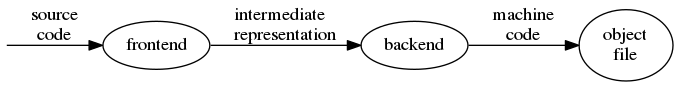
\includegraphics[width=\textwidth]{img/compiler.png}
\begin{description}[nosep]
\item[frontend] compiler part translates source code written in some programming
language syntax into IR: there are \emph{many frontends for multiple input
languages}, but \emph{single shared IR} which can be understood by any backend
\item[backend] do IR optimization and generates IR into machine code: the same
IR, and \emph{multiple target} processors
\end{description}

\clearpage\noindent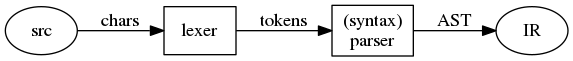
\includegraphics[width=\textwidth]{img/frontend.png} 
\begin{description}[nosep]
\item[lexer] scans input stream contains single chars of source code, and group
them into tokens: every token contains a single symbol \emph{value}, \emph{type}
tag, and location where it placed in the source code (name of a file, line
number,..). As you can see, token structure is very close to our
\verb|<type:value>| base object structure, so lexer can just return ready to use
objects.
\item[parser] eats stream of tokens and groups them into tree-like structures
according to programming language grammar. The output of parser is AST:
\term{Abstract Syntax Tree}. As \F\ has very simple sequential grammar, it does
not use syntax parser.
\end{description}

\clearpage\secrel{Lexer}\label{lexer}
\noindent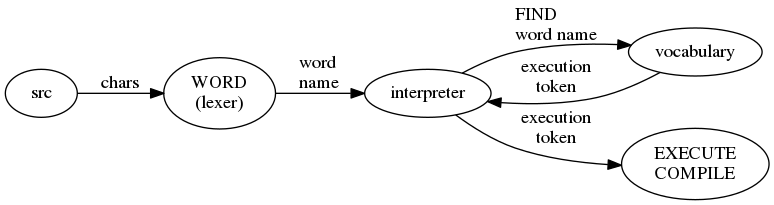
\includegraphics[width=\textwidth]{img/forthend.png} 
In classical \F\ the whole lexer is \verb|WORD| (and few words do special
lexing like \verb|\| and \verb|"| use WORD for its work). But this way has a
drawback: WORD can't distinguish word names, numbers, string and so on. If you
put 1234 in source code, \verb|WORD| returns it \emph{as string}, and
\verb|INTERPRET| must do extra work to check can it be number. If you put
\verb|" string"| you must place extra space before string content to let
interpreter first find and execute \verb|"| which will next do \verb|["] WORD|
to parse rest of string.

It is
extra easy to write classical \F\ parser in a few machine commands\note{char
reading pointer in buffer, and dumb comparing current char with spaces}, and it
is very useful in devices built on smallest microcontrollers.
But we want some \term{syntax sugar} in o\F\note{and extendable \emph{infix}
syntax in feature releases}, so we will use special parser writing library
PLY\note{and parser generators for \cpp} in place of dumb \verb|WORD|. Such
lexer will do type detection for \term{literals} (numbers, strings,..).

\clearpage
\begin{lstlisting}[language=Forth]
# metasystem tests
01 02.3 +04e-05 0xDeadBeef 0b1101 (lot of numbers)
? . ?														\ dump/clear stack
\end{lstlisting}
Here the sample code contains various types of comments, numbers, debug
\verb|?| stack dump and stack clean \verb|.| dot word. We will process it using
well known \href{http://www.dabeaz.com/ply/}{PLY library}\note{\$ sudo pip
install ply} for \py.
\begin{lstlisting}[language=Python]
############################################ lexer
import ply.lex as lex
\end{lstlisting}
We don't use \verb|ply.yacc| because lexer is enough for o\F. You can use it for
more complex recursive syntax like parens or lists.
\clearpage\noindent
ply.lex requires some predefined elements must be declared:

\begin{lstlisting}[language=Python]
# lexer error callback
def t_error(t): raise SyntaxError(t)
\end{lstlisting}
\begin{lstlisting}[language=Python]
# ignored chars: spaces
t_ignore = ' \t\r\n'
\end{lstlisting}
\begin{lstlisting}[language=Python]
def t_COMMENT(t):
    r'\#.+'
\end{lstlisting}
\begin{lstlisting}[language=Python]
# list of used token (literal) types
tokens = ['WORD','integer','number','hex','bin']
\end{lstlisting}
\clearpage\noindent
Every lexer rule should be defined in form of specially formatted function,
contains \emph{regular expression in its docstring}, and returns any object has
\verb|.type| and \verb|.value| properties. If rule function does not return any
value, a parsed element will be omitted, as it was done with \verb|t_COMMENT|.
The order of rule definition is the topmost first: \emph{earlier defined rule
has more priority}.

\medskip
\begin{lstlisting}[language=Python]
def t_NUMBER_exp(t):	# float in exponential form
	r'[\+\-]?[0-9]+(\.[0-9]*)?[eE][\+\-]?[0-9]+'
	return Number(t.value)
def t_NUMBER_point(t):					# float with point
	r'[\+\-]?[0-9]+\.[0-9]*'
	return Number(t.value)
\end{lstlisting}
\clearpage
\noindent \verb|Hex|adecimal and \verb|Bin|ary numbers are widely used in
low-level programming and HDL\note{Hardware Description Languages\ --- Verilog,
VHDL}, here we use some machine number classes:
\begin{lstlisting}[language=Python]
def t_HEX(t):							# machine number in hex
    r'0x[0-9a-fA-F]+'
    return Hex(t.value)
def t_BIN(t):									# binary bit string
    r'0b[01]+'
    return Bin(t.value)
def t_INTEGER(t):								# generic integer
    r'[\+\-]?[0-9]+'
    return Integer(t.value)
\end{lstlisting}
\clearpage\noindent o\F\ has many variants of comments in syntax:
\begin{lstlisting}[language=Python]
def t_COMMENT_hash(t):			# single line #comment
	r'\#.+'
def t_COMMENT_slash(t):			# single line \comment
	r'\\.+'
def t_COMMENT_parens(t):		# block (comment)
	r'\(.*?\)'
\end{lstlisting}

\bigskip\noindent And finally \emph{the most important lexer rule}:
\begin{lstlisting}[language=Python]
def t_WORD(t): 					# parse generic word name
    r'[a-zA-Z0-9_\?\.]+'
    return Symbol(t.value)
\end{lstlisting}
\clearpage\noindent To get results of lexer run isolated from INTERPET you can
use this code:

\begin{lstlisting}[language=Python]
lexer = lex.lex()										# create lexer
lexer.input(open('src.src').read())	# feed source
while True:													# infty loop
    token = lex.token()
    if not token: break				# until empty token
    print token
\end{lstlisting}
\begin{lstlisting}
<integer:-1>			<number:2.3>		<number:4e-05>
<hex:0xDeadBeef>	<bin:0b1101>		<symbol:?>	
<symbol:.>				<symbol:?>
\end{lstlisting}

\secrel{WORD FIND INTERPRET loop}
\emph{Non-standard WORD word} is analog of classical \verb|WORD|, but does not
get delimiter char codes from stack for its work, as it uses lexer
defined before \ref{lexer}:
\begin{lstlisting}[language=Python]
lexer = lex.lex()              		 # create lexer
							# feed stdin as source input stream
lexer.input(sys.stdin.read())

def WORD():
	token = lex.token() ; if not token: sys.exit(0)
	D << token	# push to data stack
W << WORD
\end{lstlisting}
\clearpage\noindent
\begin{lstlisting}[language=Python]
test_STRING_4Interpreter = '''
\end{lstlisting}
\begin{lstlisting}[language=Forth]
# line comment
\ slash line comment
( block comment )
ThisMustBeFirst
-01 002.3 +04e-05 0xDeadBeef 0b1101 ( lot numbers )
#this tightly inputted code can't be parsed 
\by classical FORTH, lexer only
(And)Some\Symbols
\end{lstlisting}
\begin{lstlisting}[language=Python]
'''
\end{lstlisting}
Testing of an interpreter may be some complex: we need to prepare a bit complex
source code, which must be processed several times by several parts: single
lexer alone, interpreter, and compiler.
\begin{lstlisting}[language=Python]
def test_WORD():
	lexer.input(test_STRING_4Interpreter)
	assert WORD().head() == '<symbol:ThisMustBeFirst>'
	assert WORD().head() == '<integer:-1>'
	assert WORD().head() == '<number:2.3>'
	assert WORD().head() == '<number:4e-05>'
	assert WORD().head() == '<hex:0xDeadBeef>'
	assert WORD().head() == '<bin:0b1101>'
	assert WORD().head() == '<symbol:Some>'
\end{lstlisting}
    

\clearpage\noindent
\begin{lstlisting}[language=Python]
def INTERPRET():
    while True:						# interpreter REPL loop
        WORD()						# Read
		# search/execute/compile magic should be there
        print D						# Print (stack)
W << INTERPRET
INTERPRET()			# start on VM run
\end{lstlisting}
\begin{lstlisting}
<stack:DATA>		# you will see rising stack in log
	<integer:-1>
	<number:2.3>
	<number:4e-05>
	<hex:0xDeadBeef>
\end{lstlisting}
\clearpage\noindent

\begin{lstlisting}[language=Python]
def EXECUTE():	D.pop().execute()
def FIND():			WN = D.pop() ; D << W[WN.value]
def INTERPRET():
	while True:									# interpreter loop
		WORD() # ( -- token )					# Read
		if D.top().type == 'symbol':	# ? need lookup
			FIND()    # ( token -- xt )	# Decode
			EXECUTE() # ( xt -- )				# Eval
		print D												# Print
\end{lstlisting}
If \verb|WORD| returns symbol, \term{lookup} in vocabulary must be done.
\verb|FIND| pops \term{word name} from data stack $\rightarrow$\verb|WN|, and do
search in \verb|W[]|. Resulting \term{execution token} \ref{xt} will be
\verb|EXECUTE|d.


\secup
